\chapter{Animal Kingdom}
\label{ch:animal_kingdom}

\begin{marginfigure}
    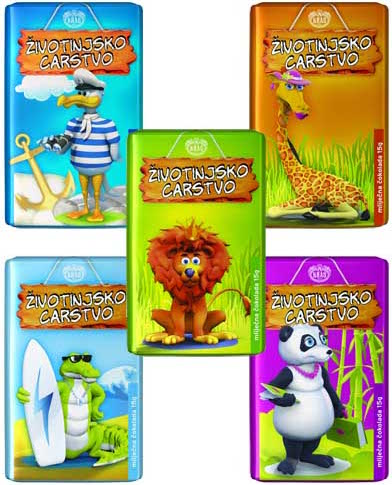
\includegraphics[width=5cm]{graphics/ch-animal_kingdom/kras_zivotinjsko_carstvo.jpg}
\end{marginfigure}

Your lecturers spent a substantial part of their youth admiring a particular Croatian chocolate called Animal Kingdom. Each chocolate bar came with a card---a drawing of some (random) animal, and the associated album made us eat a lot of chocolate.

Funny stuff was we never understood the order in which the cards were laid out in the album. We later learned about taxonomy, but being more inclined to engineering we never mastered learning it in our biology classes. Luckily, there’s data mining and the idea that taxonomy simply stems from measuring the distance between species.

\begin{wrapfigure}{o}{0.8\textwidth}
    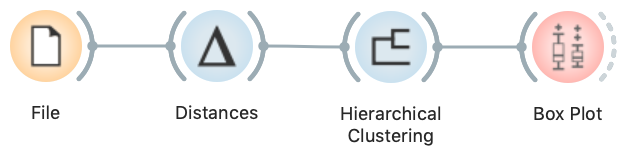
\includegraphics[scale=0.4]{graphics/ch-animal_kingdom/workflow.png}
    \caption{Hierarchical clustering works fast for smaller data sets. But for bigger ones it fails. Simply, it cannot be used. Why?}
\end{wrapfigure}

Here we use zoo data (from the documentation data sets) with attributes that report on various features of animals (has hair, has feathers, lays eggs). We measure the distance and compute the clustering. Animals in this data set are annotated with type (mammal, insect, bird, and so on). It would be cool to know if the clustering re-discovered these groups of animals.

To split the data into clusters, let us manually set a threshold by dragging the vertical line left or right in the visualization. Can you say what is the appropriate number of groups?

\begin{figure*}[h]
    \centering
    \newcommand{\clustering}{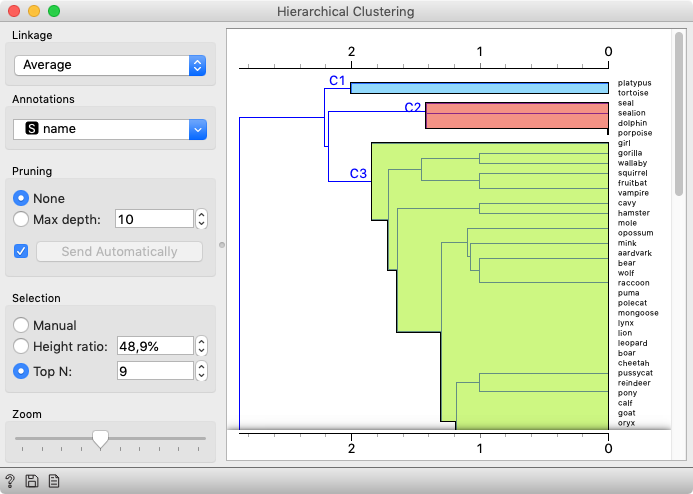
\includegraphics[scale=0.35]{graphics/ch-animal_kingdom/clustering.png}}
    \newcommand{\plot}{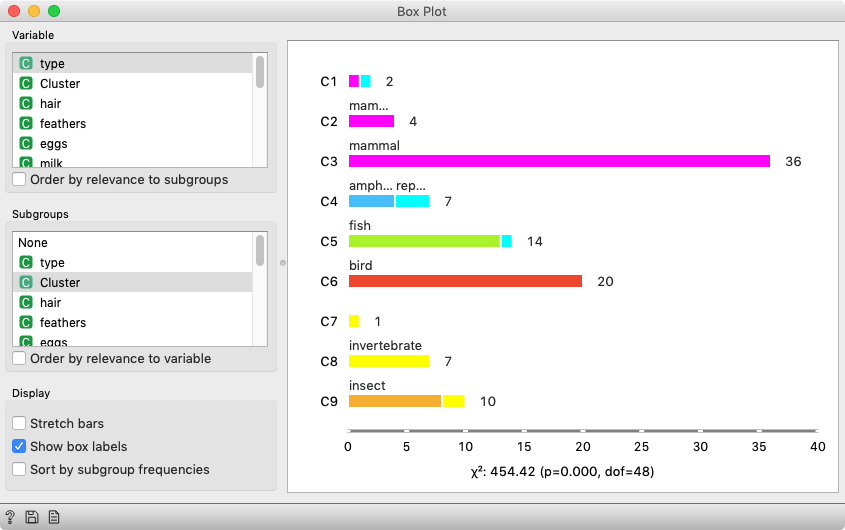
\includegraphics[scale=0.35]{graphics/ch-animal_kingdom/boxplot.png}}
    \infinitewidthbox{
    \stackinset{r}{-0.5\linewidth}{t}{+0.1\linewidth}{\plot}{\clustering}\hspace{8cm}
    }
    \caption{What is wrong with those mammals? Why can't they be in one single cluster? Two reasons. First, they represent 40\% of the data instances. Second, they include some weirdos. Who are they?}
\end{figure*}

